\documentclass{article}
\usepackage[utf8]{inputenc}

%%Let's you change margins
\usepackage[left=1in,right=1in,top=1in,bottom=1in]{geometry}

%%Math symbols, proof environments
\usepackage{amsmath,amsthm,amssymb, graphicx}
\usepackage{subcaption}
\newcommand{\atan}{\tan^{-1}}

%%Use this package for matrices
\usepackage{array}

%%Commands for common sets
\newcommand{\R}{\mathbb{R}} %Real numbers
\newcommand{\Z}{\mathbb{Z}} %Integers

\title{ECE 141 Project} %Remove Template in your title

\author{Inesh Chakrabarti} %Put your name here

\date{\today}

\begin{document}

\maketitle

\subsection*{Problem 1}
Show that for any desired $\beta$ in $[0, 2\pi)$ there exists a $u$ in $[0, 2\pi)$ so that (5) holds. We can thus treat $\beta$ as the input since for any $\beta$ computed by a controller we can compute the steering angle $u$ via the relation (5) and apply this command to the motor steering for the wheels. This will greatly simplify the equations you have to work with.
\begin{proof}[Solution]
First, let us look at relation (5):
\[\beta = \atan\left(\dfrac{\ell_r}{\ell_r+\ell_f}\tan(u)\right)
\]
Note that we know $\ell_f = 1.1m$ and $\ell_r = 1.7m$, so subsitututing, we are left with 
\[\beta = \atan\left(\dfrac{1.7}{1.7+1.1}\tan(u)\right)= \atan(k\tan(u))
\]
where $k=\dfrac{1.7}{2.8} \approx 0.607142857$ \newline
Note that the range of $tan(u)$ for $u \in [0, 2\pi)$ is all real numbers, so the range of $ktan(u)$ must also be all real numbers. Therefore, we can deal with $\atan$ function's regular range, as we have included all numbers in its domain. Assuming that the given $\atan$ refers to a four quadrant tangent inverse function, we thus arrive at the conclusion that for any desired $\beta \in [0, 2\pi)$ there exists some $u \in [0, 2\pi)$
\end{proof}

\subsection*{Problem 2}
We first consider the lane keeping problem, i.e., the design of a controller that keeps the car in the center of its lane. For this purpose we assume the car’s velocity to be constant at 35 mph, that the lane center corresponds to $y = 0$, and that we have a sensor measuring $y$ (in reality, the position of the car on the lane would be computed by using vision to detect the location of the lane markers). Linearize the equations of motion and design a controller that stabilizes the car at $y = 0$ using the linearized model (use the transfer function from $\beta$ to $y$). You don’t need to work with equation (1) since $x$ will not be at equilibrium. Provide some plots showing the controller works as intended.
\begin{proof}[Solution]

First we note that the equations we must linearize are:
\[\dot{y} = v\sin(\psi+\beta)
\]
\[\dot{\psi} = \frac{v}{\ell_r}\sin(\beta)
\]
Let us now try to find a value to linearize these equations around. It makes sense to linearize these equatoins around $\psi = 0$ and $\beta = 0$, as most of our values for these two angles will fall near these values, especially since we are trying to straighten teh car in the lane.
\newline
Then, we can use the small-angle approximation, which holds true around $0$, use the approximations:
\[\sin(\psi+\beta) \approx \psi+\beta 
\]
\[\sin(\beta) \approx \beta
\]
Thus, our linearized equations are:
\[\dot{y} = v(\psi + \beta)
    \]
\[\dot{\psi} = \frac{v\beta}{\ell_r}
    \]
Note that the velocity of the car for this question is $35$ mph, which is the same as $15.6464$ m/s. We can also calculate $\frac{v}{\ell_r}=\frac{15.6464}{1.7}=9.2038$. \newline
Now, let us determine what it means for the controller to work as intended. For the controller to work as intended, we must haev that the car does not respond too fast; this means that it should not jerk immediately to correct itself. Thus, we can set a constraint for $t_r > 0.1$s, except for specific cases where it is normal for correction to occur very fast (such as when y = 0 and only the angle is different). However, we also want to minimize overshoot to some value, as the car may swerve with excessive overshoot, which is undesirable. Thus, let us arbitarily set a maximum overshoot of $0.5$m, which is about half a meter, an amount most people would be comfortable having the car adjust by. However, I will limit the car to one noticable oscillation, where noticable is any oscillation above 0.1. \newline
Let us now determine what valid inital conditions for $y$ and $\psi$ would be. It makes sense to limit $y$ to small values. Considering the next question uses lanes $3$ m wide, let us use $y \in [-1.5,1.5]$. Similarily, let us consider the range for $\psi$. Similarily, we can arbitarily decide $\psi \in \left[-\frac{pi}{3},\frac{pi}{3}\right]$, which is approximately $\psi \in [-1,1]$. Now we can use simulink to simulate our model. \newline

\begin{figure}[h!]
    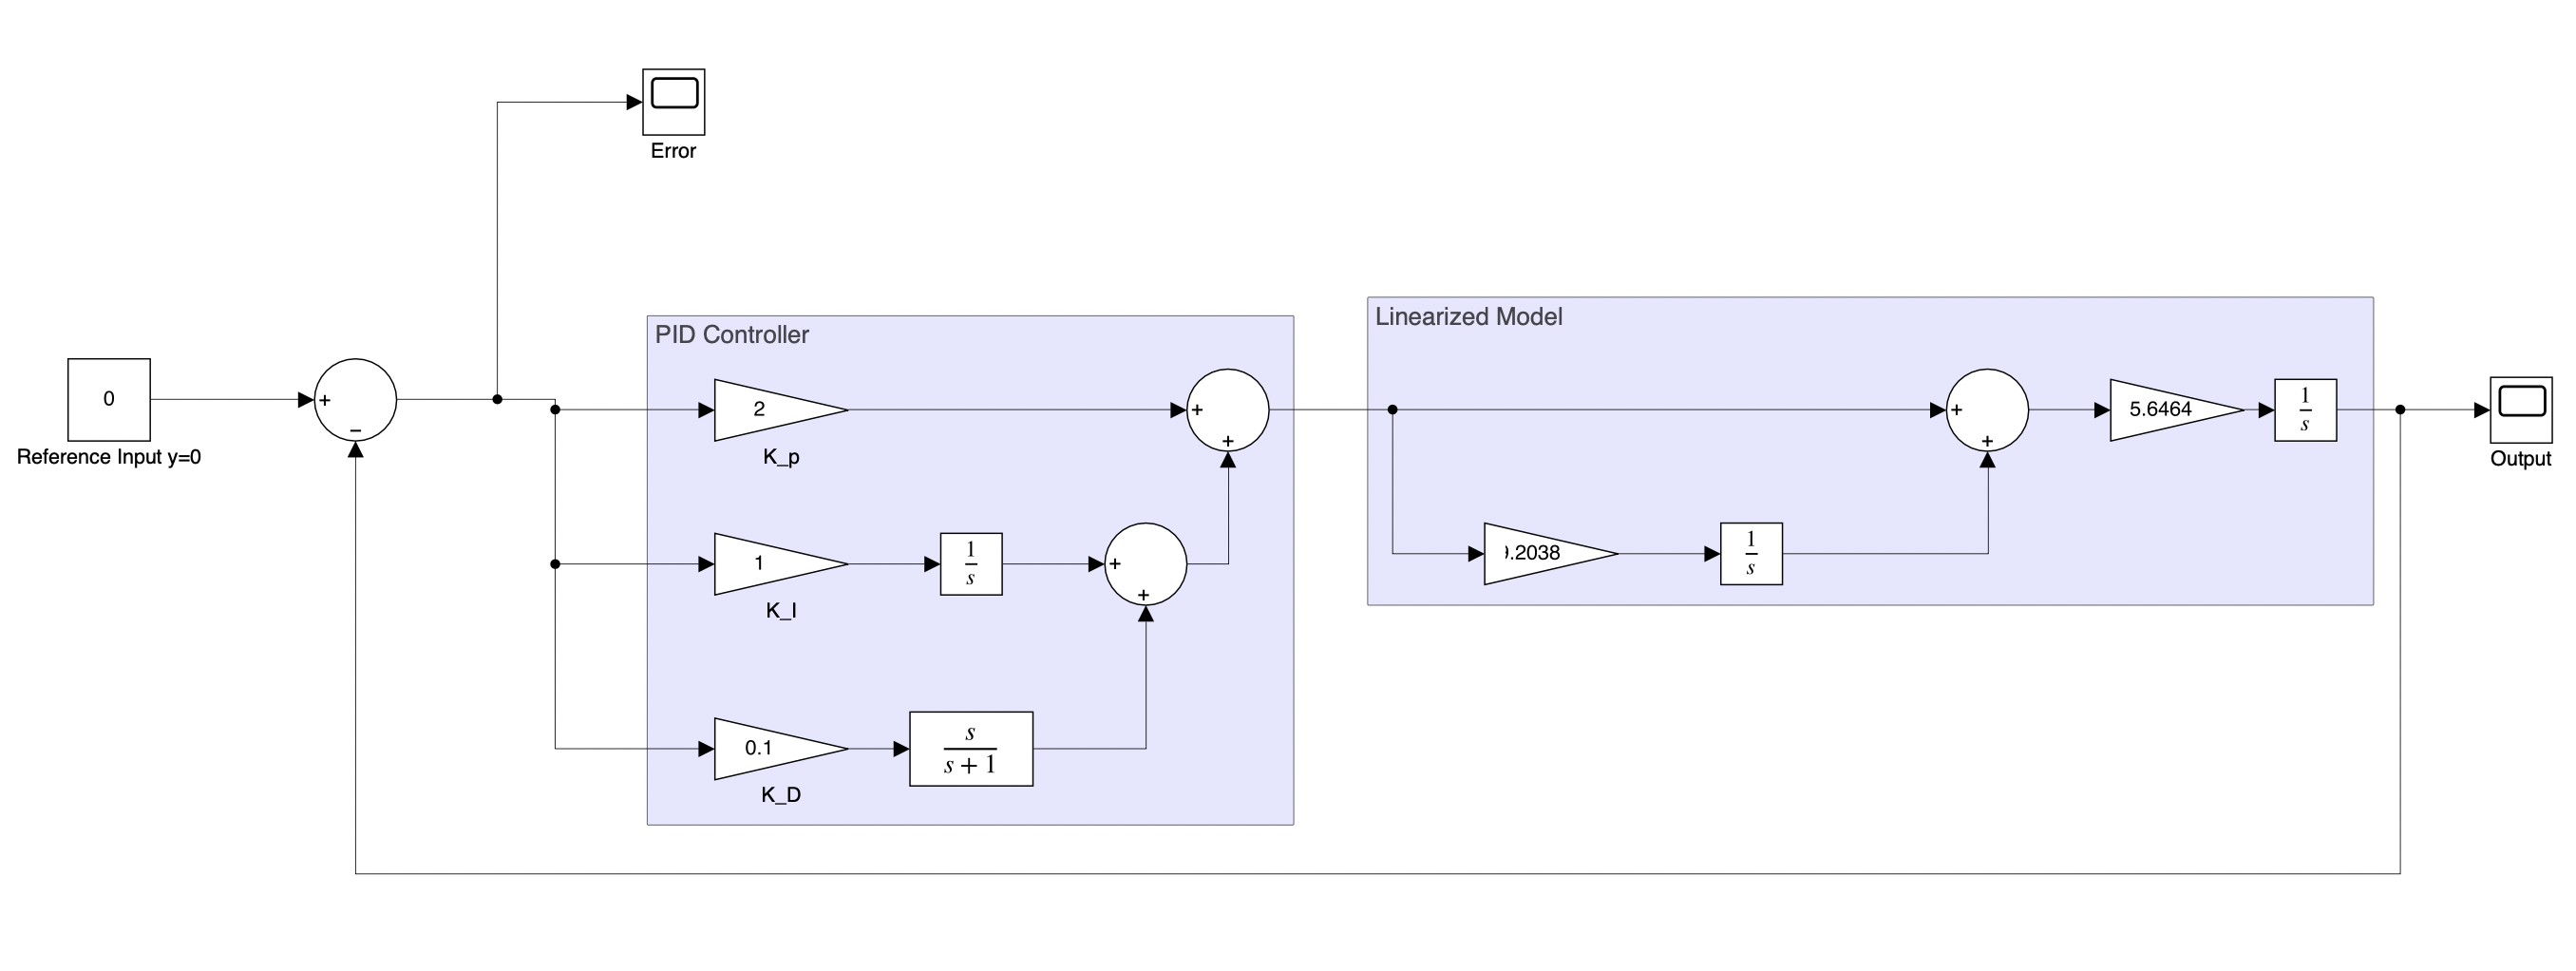
\includegraphics[width=\linewidth]{ECE141Q2Model.png}
    \caption{Linearized Simulink Model}
\end{figure}

Figure 1 dispalys the simulink block diagram we used for our linearized model. Note that we have used a PID controller. 
Now let us apply inputs to this controller to different initial conditions to observe the controller behavior:
\begin{figure}[h!]
    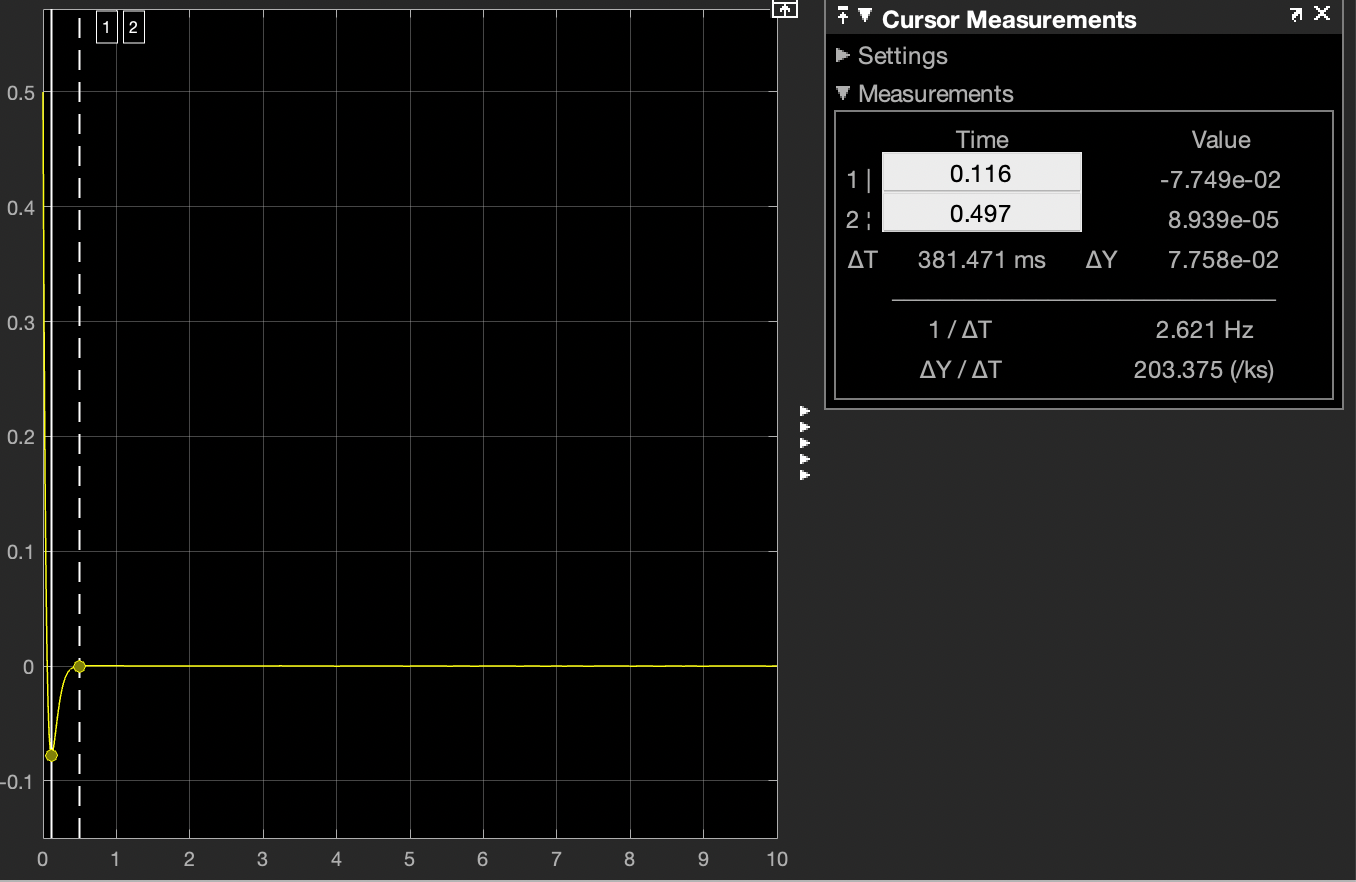
\includegraphics[width=\linewidth]{img1.png}
    \caption{Step Response for Controller}
\end{figure}
First, note that there is zero steady state error with a step input in unity feedback. We also see that it meets all of our required conditions. Next, let us observe the controller's response to differnet initial conditions. 
\newpage
\begin{figure}[h]
    \centering
    \begin{subfigure}{0.4\linewidth}
      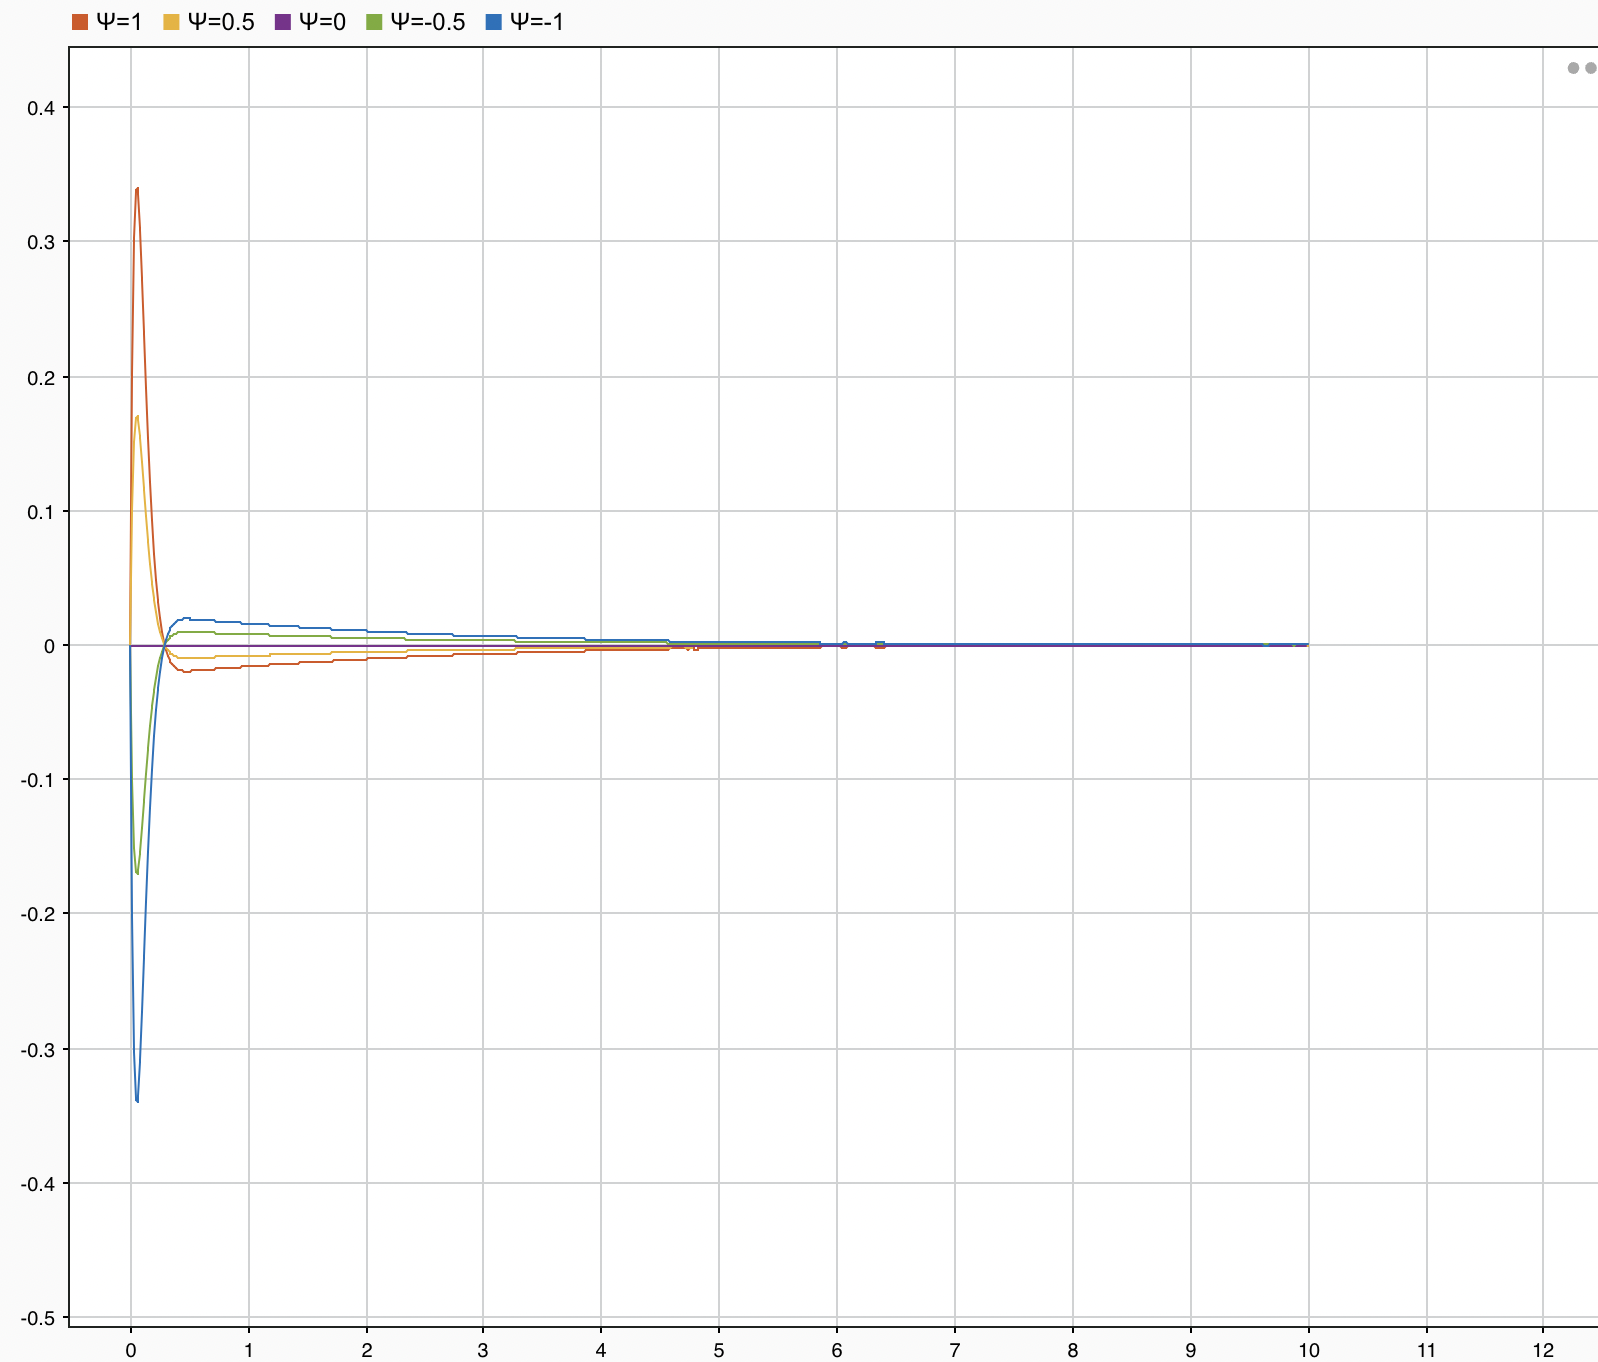
\includegraphics[width=\linewidth]{img2.png}
      \caption{Plots for y=0}
    \end{subfigure}
    \begin{subfigure}{0.4\linewidth}
      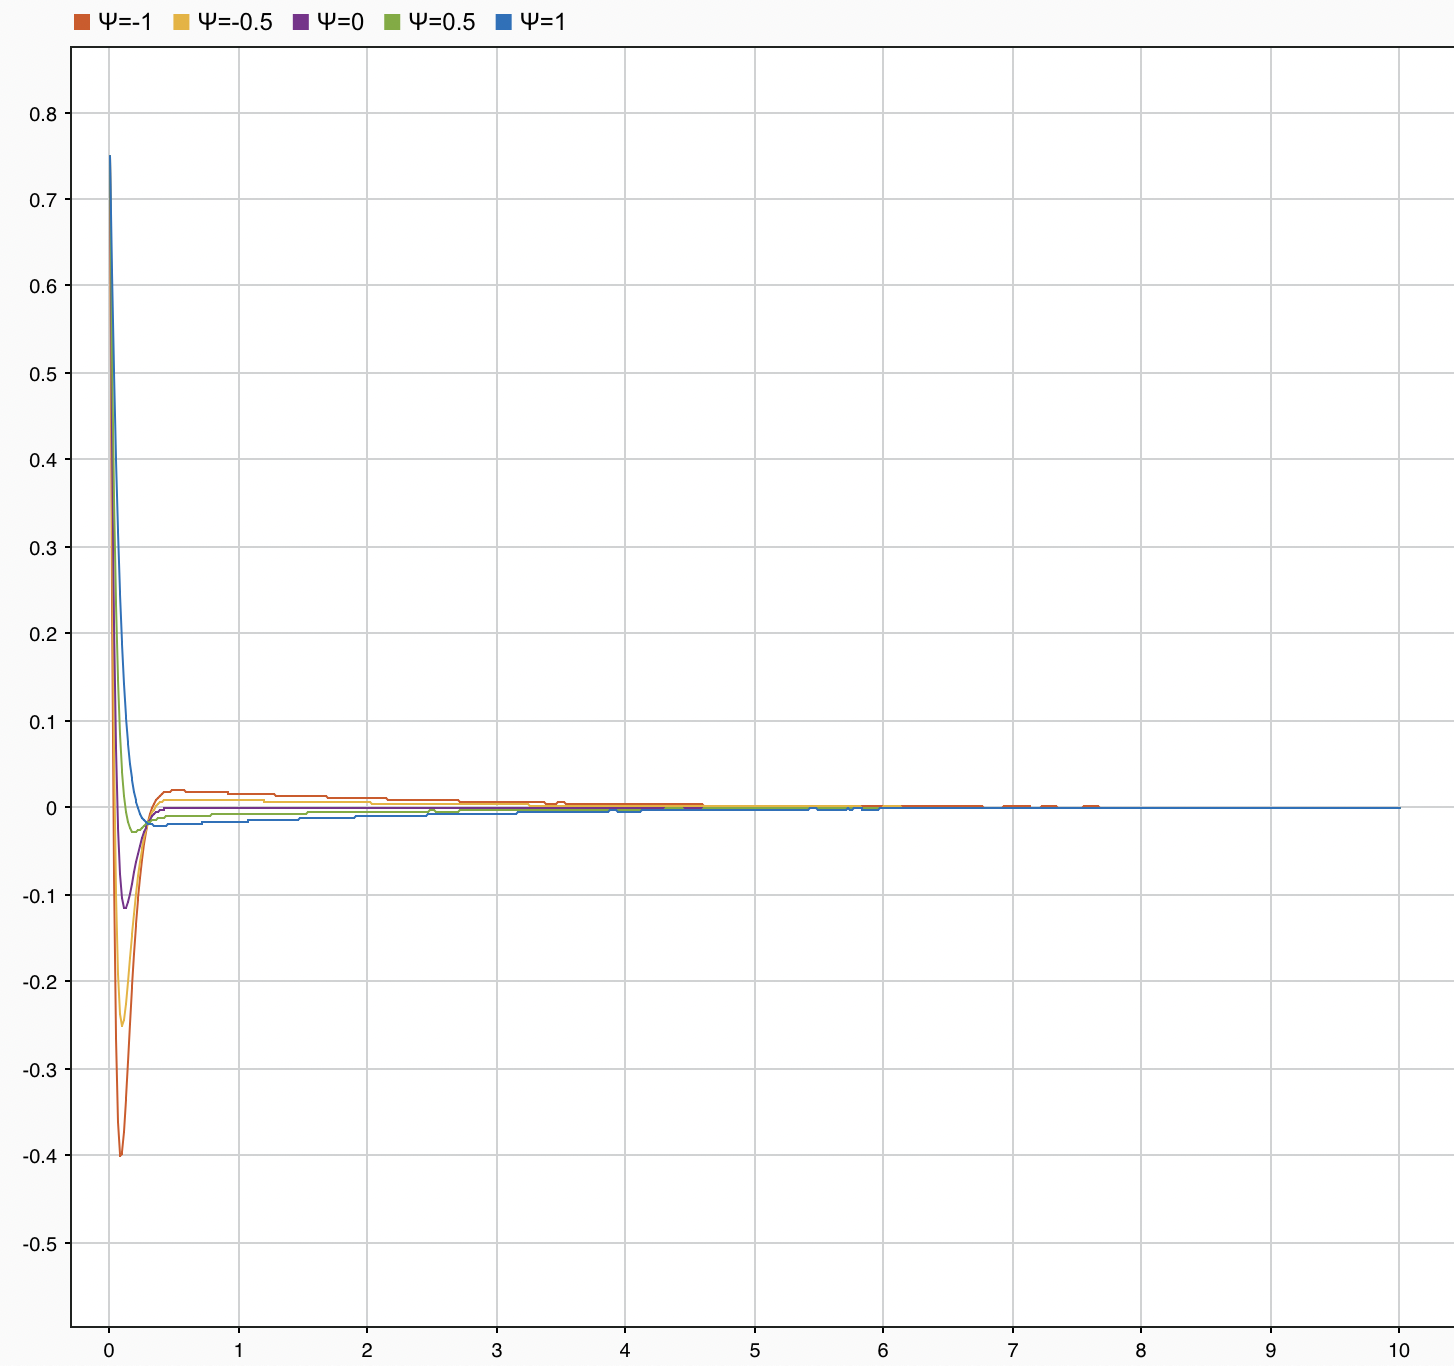
\includegraphics[width=\linewidth]{img3.png}
      \caption{Plots for y=0.75}
    \end{subfigure}
    \begin{subfigure}{0.4\linewidth}
        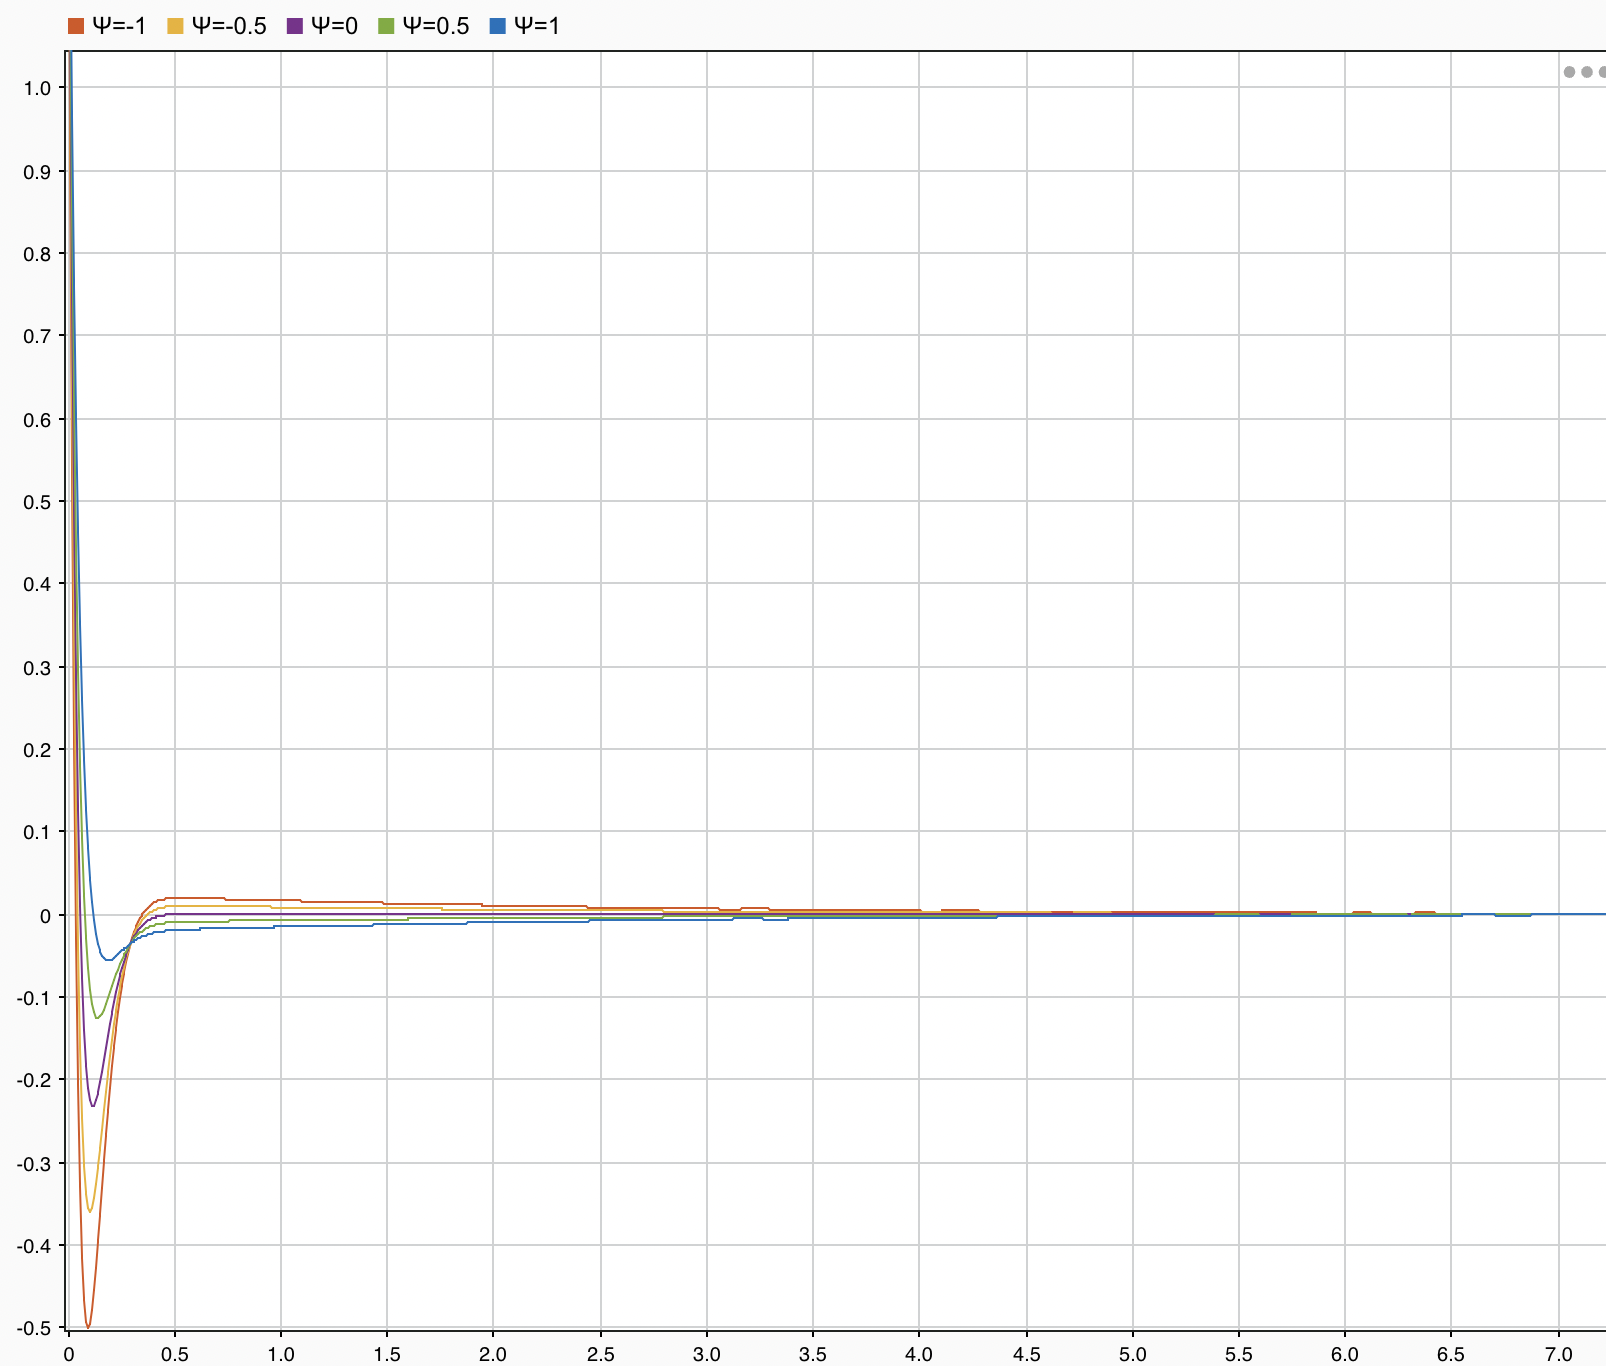
\includegraphics[width=\linewidth]{img4.png}
        \caption{Plots for y=1.5}
      \end{subfigure}
      \begin{subfigure}{0.4\linewidth}
        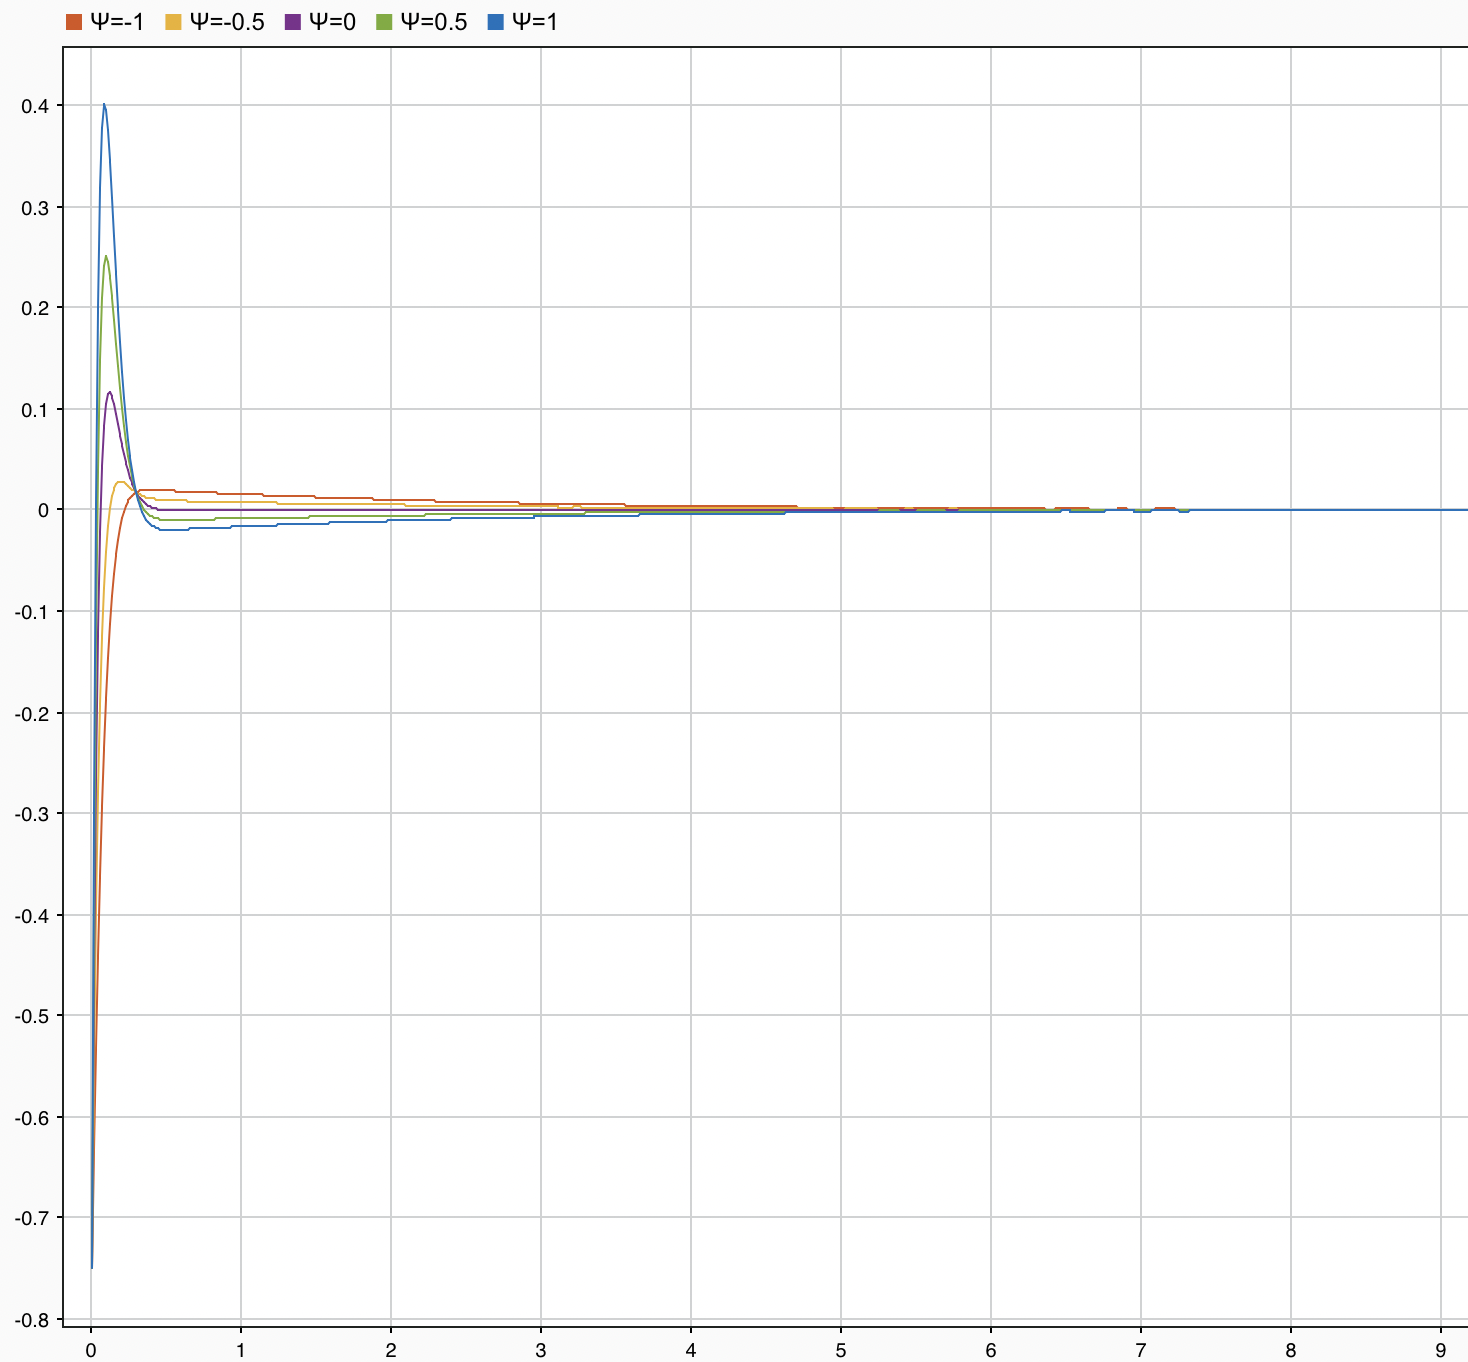
\includegraphics[width=\linewidth]{img5.png}
        \caption{Plots for y=-0.75}
      \end{subfigure}
      \begin{subfigure}{0.4\linewidth}
          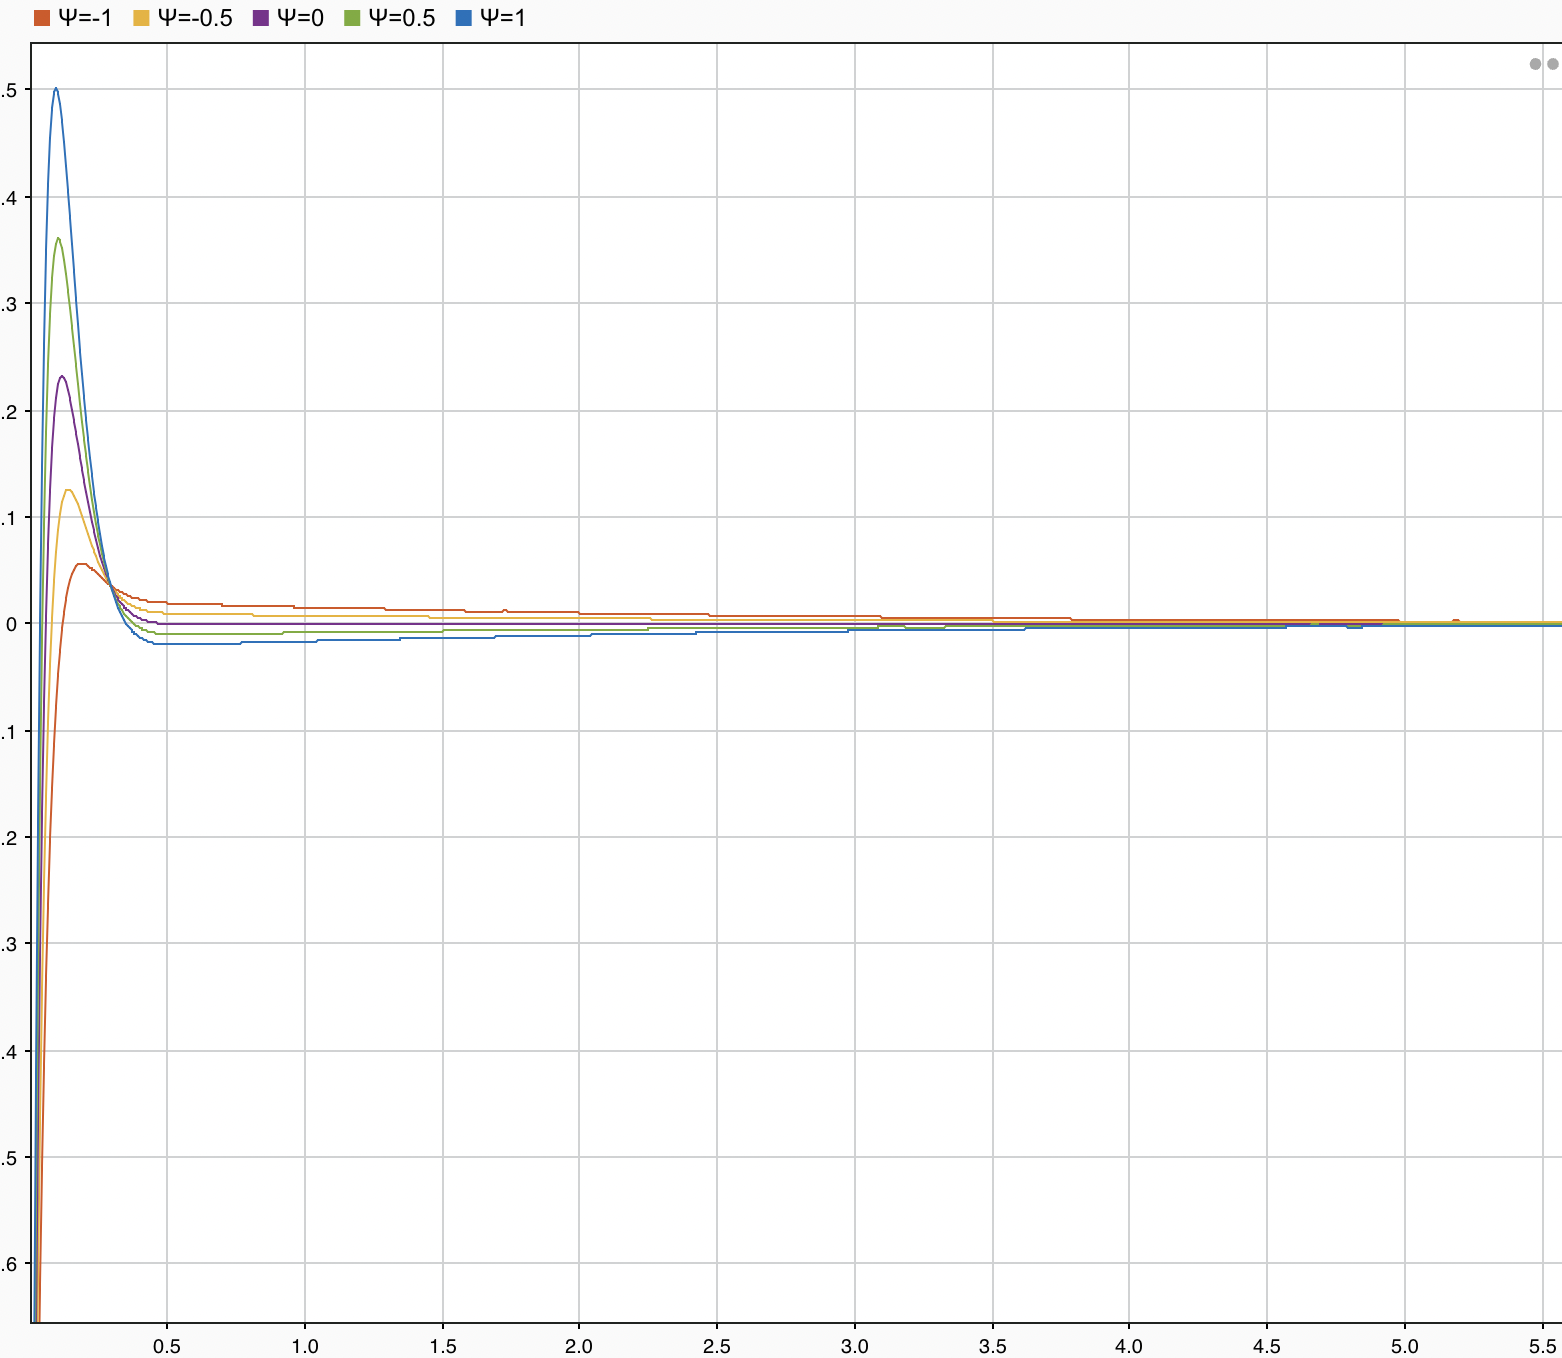
\includegraphics[width=\linewidth]{img6.png}
          \caption{Plots for y=-1.5}
        \end{subfigure}
    \caption{Plots for different initial conditions}
    \label{fig:coffee}
  \end{figure}
We note that our controller does work as intended and meet all of our conditions.
\end{proof}
\end{document}

